\documentclass{article}
\usepackage{graphicx} % Required for inserting images
\usepackage{caption}
\usepackage[utf8]{inputenc}
\usepackage[style=authoryear, backend=biber]{biblatex}
\addbibresource{refs.bib} % Reference file

\title{Variation of Pollutants in 2025 in Tucson}
\author{Shruti Karandikar\\
    \small Advisor: Dr. Armin Sorooshian\\
    \small Course: ASTR 399}
\date{May 2026}
\begin{document}\maketitle

\section{Introduction}

Air pollution is an environmental and health concern in big cities around the world. The two prominent pollutants are nitrogen dioxide ($NO_2$) and formaldehyde ($HCHO$). $NO_2$ mainly comes from cars and traffic, so we can hypothesize that we would see less of it on the weekends as fewer people are driving. $HCHO$ comes both from human activities and natural chemical reactions in the air, so we can not hypothesize the same.

In this study we analyzed the levels $NO_2$ and $HCHO$ in Tucson, Arizona across different time periods. We compare our analysis with previous research in other cities.

\section{Previous Work}

Cities other than Tucson have found a consistent weekend drop for $NO_2$ \cite{HM2025, BM2021A, BM2021B}. This is because cars and traffic produce most of the $NO_2$ in urban areas, and there is less driving on weekends. For example, a research in Pune, India found that $NO_2$ has a clear traffic-induced peak at approximately 9:00 AM on weekdays \cite{BM2021B}.

Formaldehyde behaves very differently than $NO_2$. Unlike $NO_2$, $HCHO$ is not only dependent on  human activities. It is produced when sunlight reacts with gases from plants and other sources in the air \cite{BM2021A}. Because of this, the weekend effect for $HCHO$ varies. The Pune study specifically found that "both $HCHO$ and $NO_2$ do not show any considerable difference between weekdays and weekends". This means $HCHO$ doesn't follow a simple traffic pattern \cite{BM2021B}.

In Pune, researchers found that both $NO_2$ and $HCHO$ were highest in winter (October-February) and lowest during monsoon season (June-September) because the monsoon rains wash pollutants out of the air and the wet conditions affect how they are produced \cite{BM2021B}. 


\section{Experimental Methods}

We used data from a Pandora spectrometer located at the University of Arizona in Tucson \cite{GH26, PD26}. This instrument measures gases in the air using a technique called Direct Sun Spectroscopy. The spectrometer analyzes how sunlight is absorbed as it passes through Earth's atmosphere. Gases like $NO_2$ and $HCHO$ absorb light at specific wavelengths. By measuring which wavelengths of sunlight reach the instrument and which are blocked by atmospheric gases, we can determine the total amount of each gas in the air column above Tucson. Due to this we used data from 2025 focusing on daytime hours when sunlight is available (6 AM to 6 PM). 

We organized the data by five seasons Tucson has:
    \begin{itemize}
        \item DJF (Winter): December, January, February
        \item MAM (Spring): March, April, May
        \item June (Pre-Monsoon): Just June
        \item JAS (Monsoon): July, August, September
        \item ON (Post-Monsoon): October, November
    \end{itemize}
    
We separated the data into weekdays and weekends to compare pollution levels and we also looked at how levels changed throughout the day: morning (6AM –10 AM), midday (10 AM –2 PM), and afternoon (2 PM –6 PM).
The data was processed and analyzed using Python with the \texttt{pandas} library for understanding the data, \texttt{matplotlib} for \texttt{visualization}, and \texttt{seaborn} for statistical plotting. All the code is available on Github \cite{GH26}.

\section{Results and Discussion}

\subsection{Daily variations across weeks and seasons} 

\begin{figure}[t]
    \centering
    \includegraphics[width=\linewidth]{Screenshot 2026-05-16 at 8.29.16 AM.png}
    \caption{$NO_2$ Daily Variations}
    \label{fig:placeholder}
\end{figure}

$NO_2$ Weekend Drop:
$NO_2$ was consistently lower on weekends than weekdays across all seasons, dropping by 12.3\% to 16.8\%.This made sense because there is less traffic on weekends means fewer emissions from cars.

\begin{figure}[t]
    \centering
    \includegraphics[width=\linewidth]{Screenshot 2026-05-16 at 8.29.31 AM.png}
    \caption{$HCHO$ Daily Variations}
    \label{fig:placeholder}
\end{figure}

\begin{figure}[h]
    \centering
    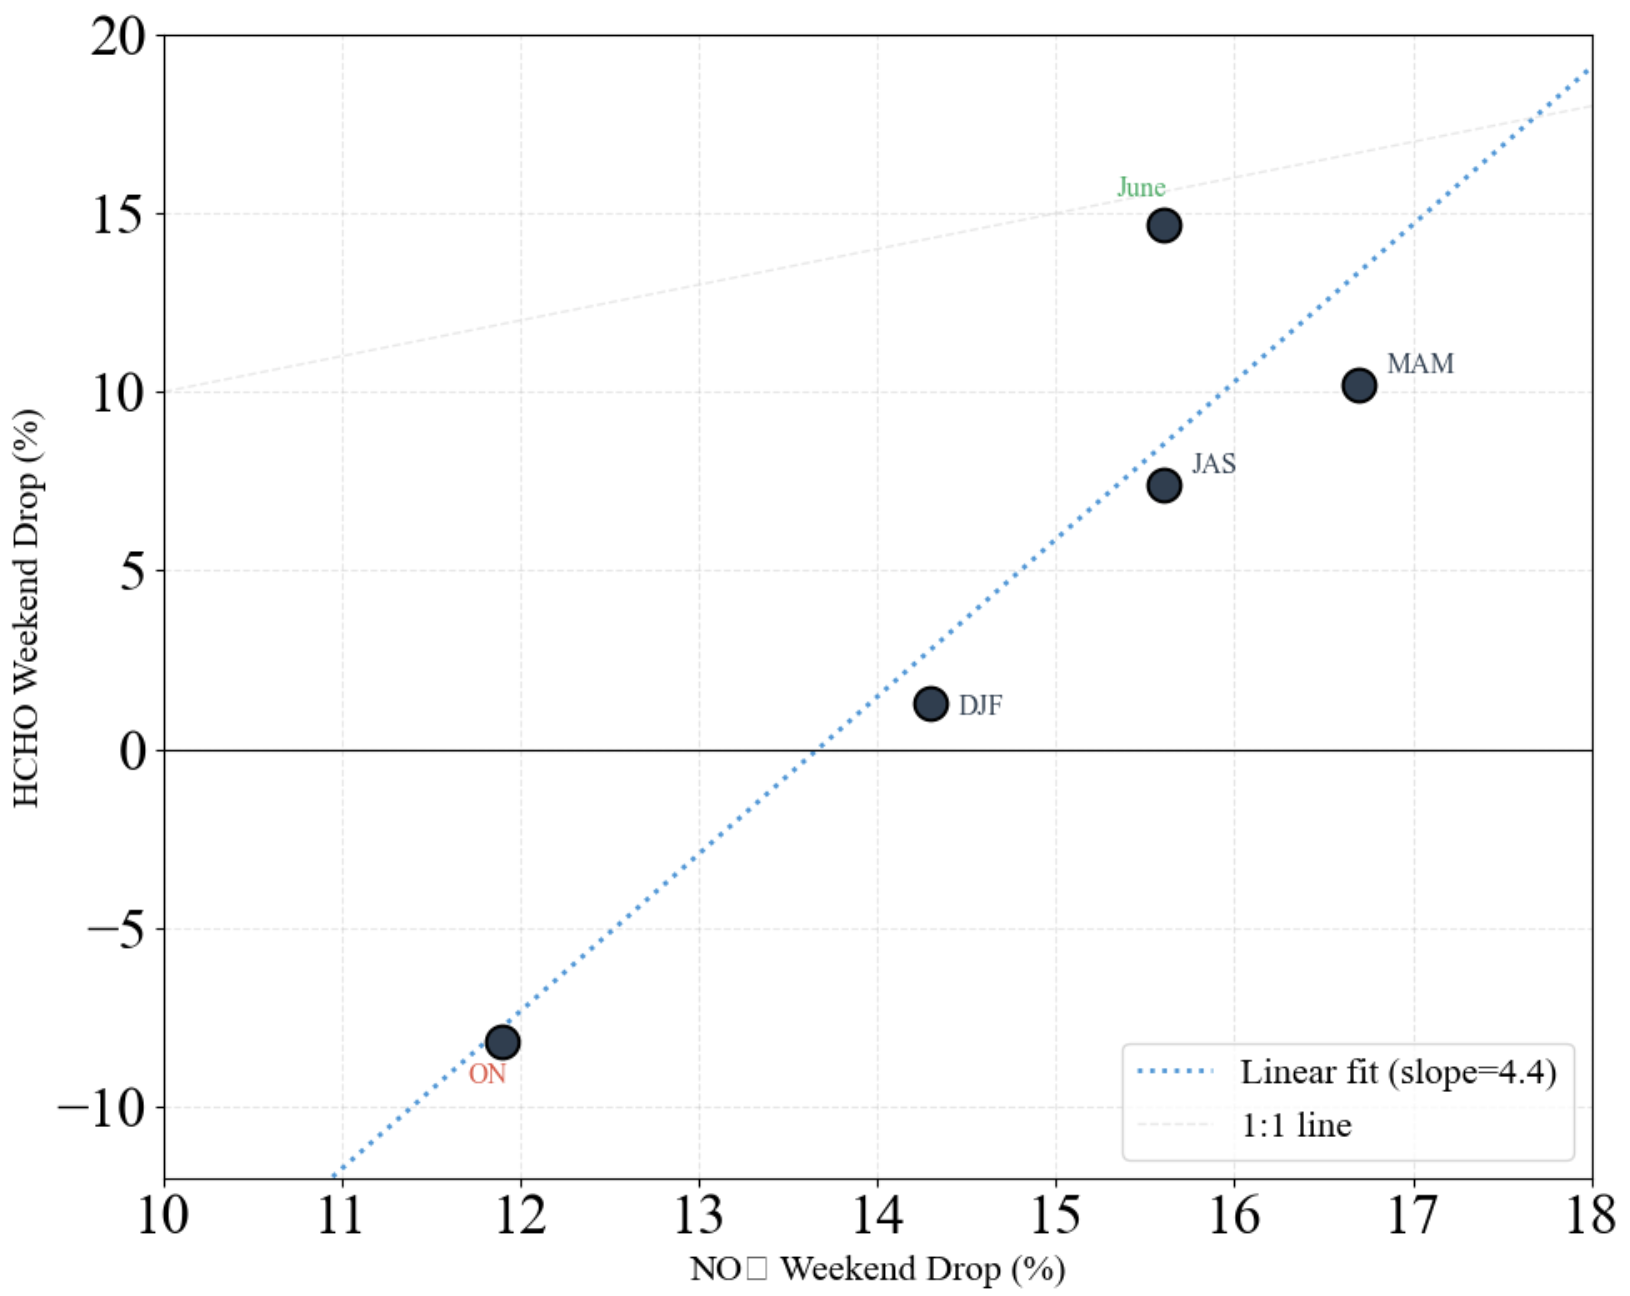
\includegraphics[width=\linewidth]{Screenshot 2026-05-16 at 8.31.57 AM.png}
    \caption{$NO_2$ vs $HCHO$ Weekend Drop by Season}
    \label{fig:placeholder}
\end{figure}


$HCHO$ Weekend Effect:
$HCHO$ behaved very differently. Its weekend pattern changed by season:

\begin{itemize}
    \item Winter (DJF): Almost no weekend effect (1.3\% drop)
    \item Spring (MAM): Moderate drop (10.2\%)
    \item June (Pre-Monsoon): Strong drop (14.7\%)
    \item Monsoon (JAS): Weak drop (7.4\%)
    \item Post-Monsoon (ON): Actual increase ($-8.2$\% means higher on weekends!)
\end{itemize}
        
The post-monsoon increase was not expected and suggested that a different chemical process is happening. We also observed that less traffic on weekends might change how ozone chemistry works in the air, actually producing more $HCHO$ instead of less.

The drop across the weekend is roughly correlated except for the outlier in June. This is possibly due to the interaction between the different sources of the pollutants.

\subsection{Hourly variations across the week and seasons} 
$NO_2$ Time-of-Day Patterns:
$NO_2$ showed the strongest weekend effect in the morning (6–10 AM) when traffic peaked. The morning rush hour weekend drop ranged from 18–22\% across seasons, which indicated that traffic is the dominant source. In contrast, the afternoon weekend drop (2–6 PM) was much weaker, ranging from only 8–13\%. Interestingly, winter (DJF) showed a more uniform weekend drop across time periods (approximately 15\% in both morning and afternoon), which could mean that there are other sources that operate throughout the day, not just during rush hours.

\begin{figure}[h]
    \centering
    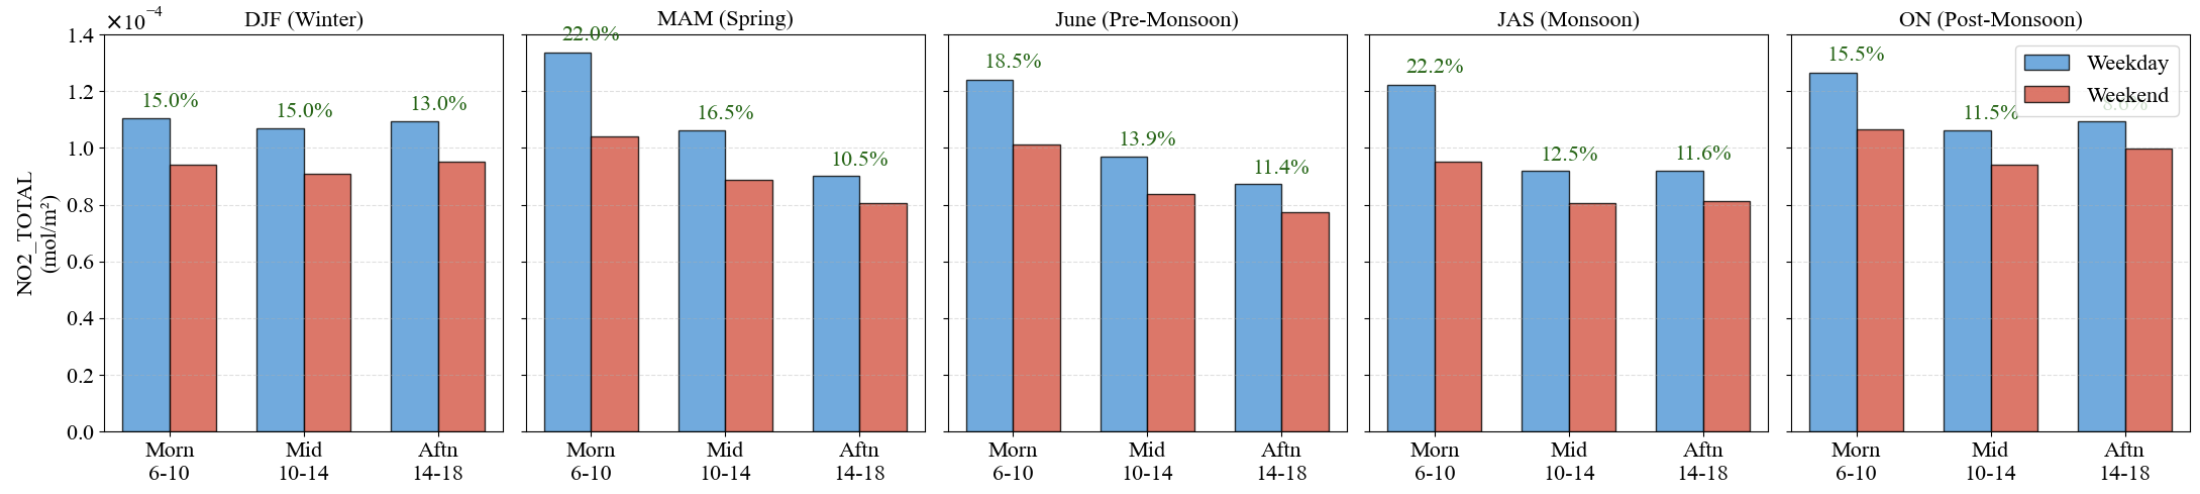
\includegraphics[width=\linewidth]{Screenshot 2026-05-16 at 8.33.38 AM.png}
    \caption{$NO_2$ Hourly Variations}
    \label{fig:placeholder}
\end{figure}

$HCHO$ Time-of-Day Patterns:
$HCHO$'s time-of-day behavior is highly season-dependent, contrasting sharply with $NO_2$. In June (pre-monsoon), $HCHO$ shows a morning weekend drop of $17.7\%$, which is similar to the $NO_2$ morning signal. The post-monsoon (ON) weekend increase in $HCHO$ is not a time-of-day phenomenon but rather an effect of chemical reactions which takes place throughout the day. This pattern suggests that afternoon biogenic VOC emissions (which peak with temperature) interact differently with weekday versus weekend $NO_x$ levels, creating conditions that actually enhance $HCHO$ formation on low-traffic weekends.

\begin{figure}[h]
    \centering
    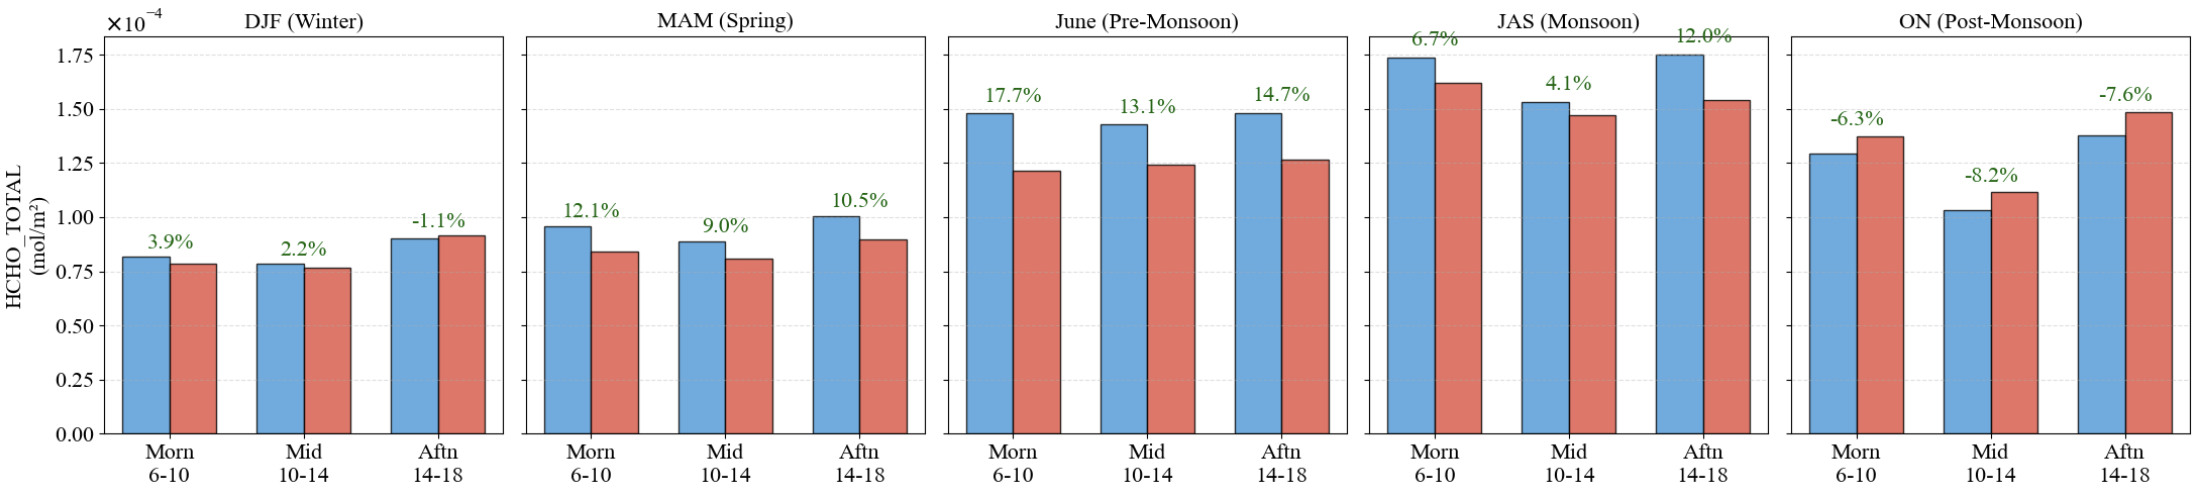
\includegraphics[width=\linewidth]{Screenshot 2026-05-16 at 8.33.55 AM.png}
    \caption{$HCHO$ Hourly Variations}
    \label{fig:placeholder}
\end{figure}

\subsection{Seasonal variation across the days and weeks}
$NO_2$ Seasonal Pattern:
The variation in the weekend drop across all seasons is more pronounced in the morning hours.

\begin{figure}[t]
    \centering
    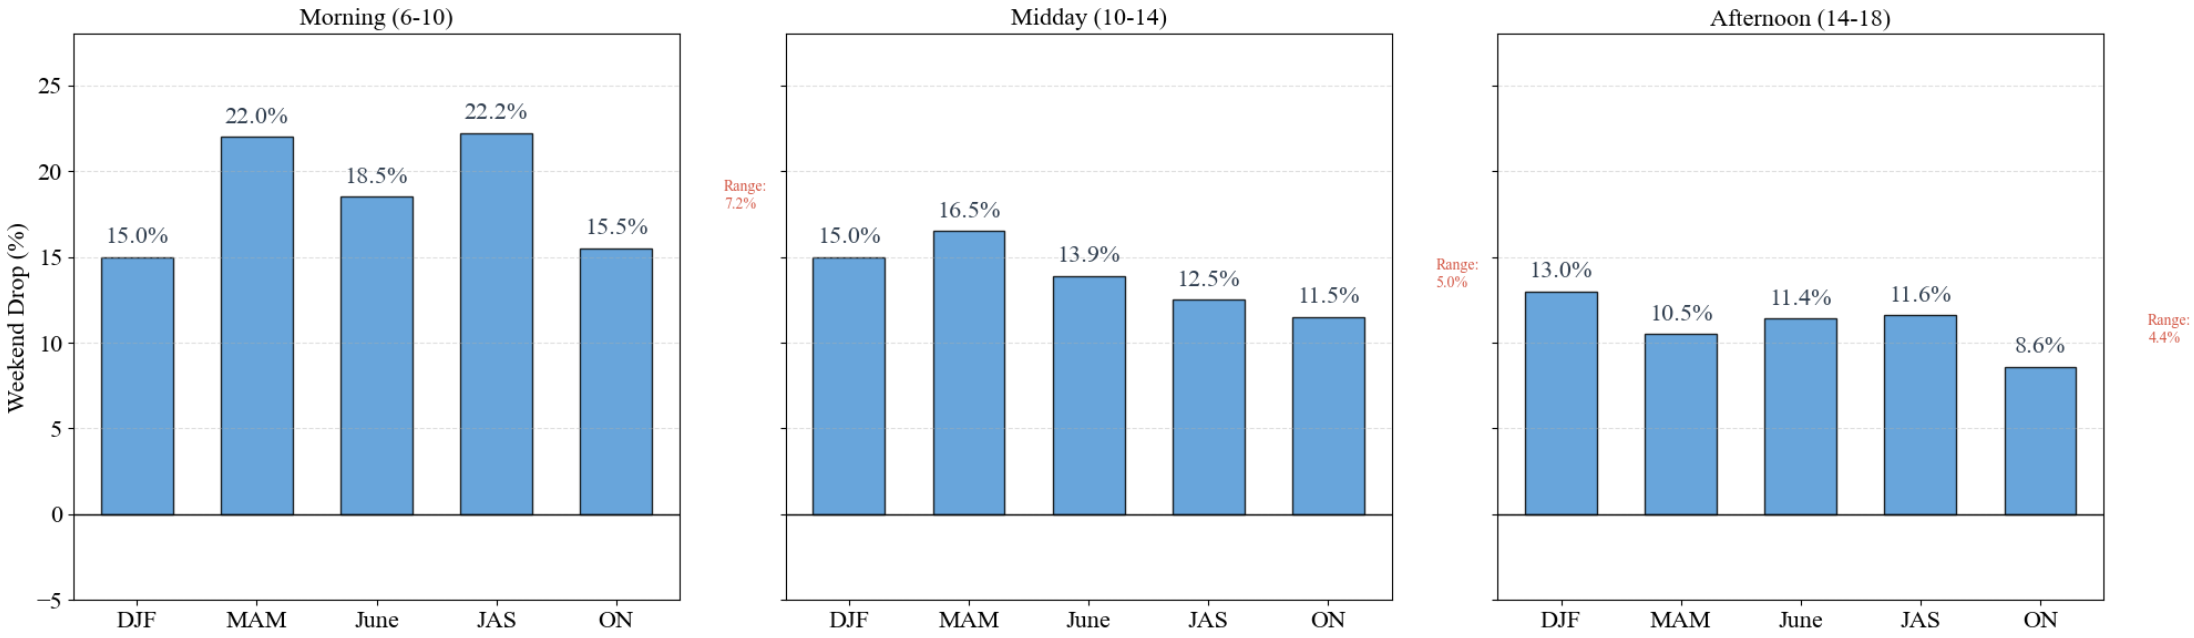
\includegraphics[width=\linewidth]{Screenshot 2026-05-16 at 8.35.24 AM.png}
    \caption{$NO_2$ Seasonal Variation}
    \label{fig:placeholder}
\end{figure}

$HCHO$ Seasonal Pattern:
The weekend level of $HCHO$ actually increases during the October-November season.

\begin{figure}[t]
    \centering
    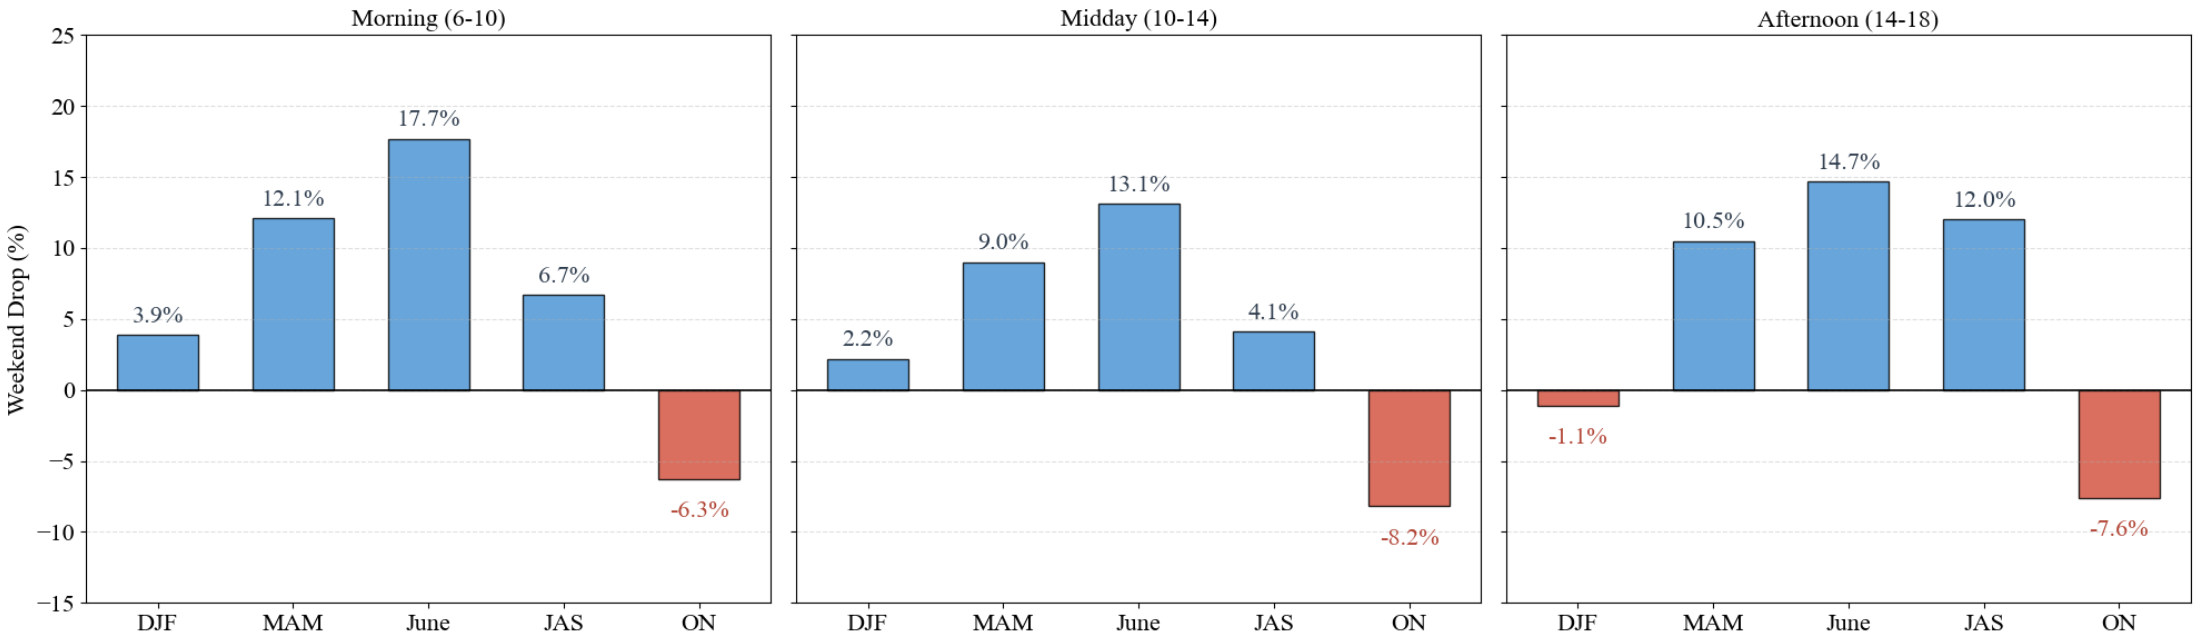
\includegraphics[width=\linewidth]{Screenshot 2026-05-16 at 8.35.36 AM.png}
    \caption{$HCHO$ Seasonal Variation}
    \label{fig:placeholder}
\end{figure}

The different behavior of $NO_2$ and $HCHO$ becomes apparent in the following figure. The weekend drop during winter and post-monsoon seasons are approximately consistent. However, in the other seasons the weekend drop varies by time of day.

\begin{figure}[t]
    \centering
    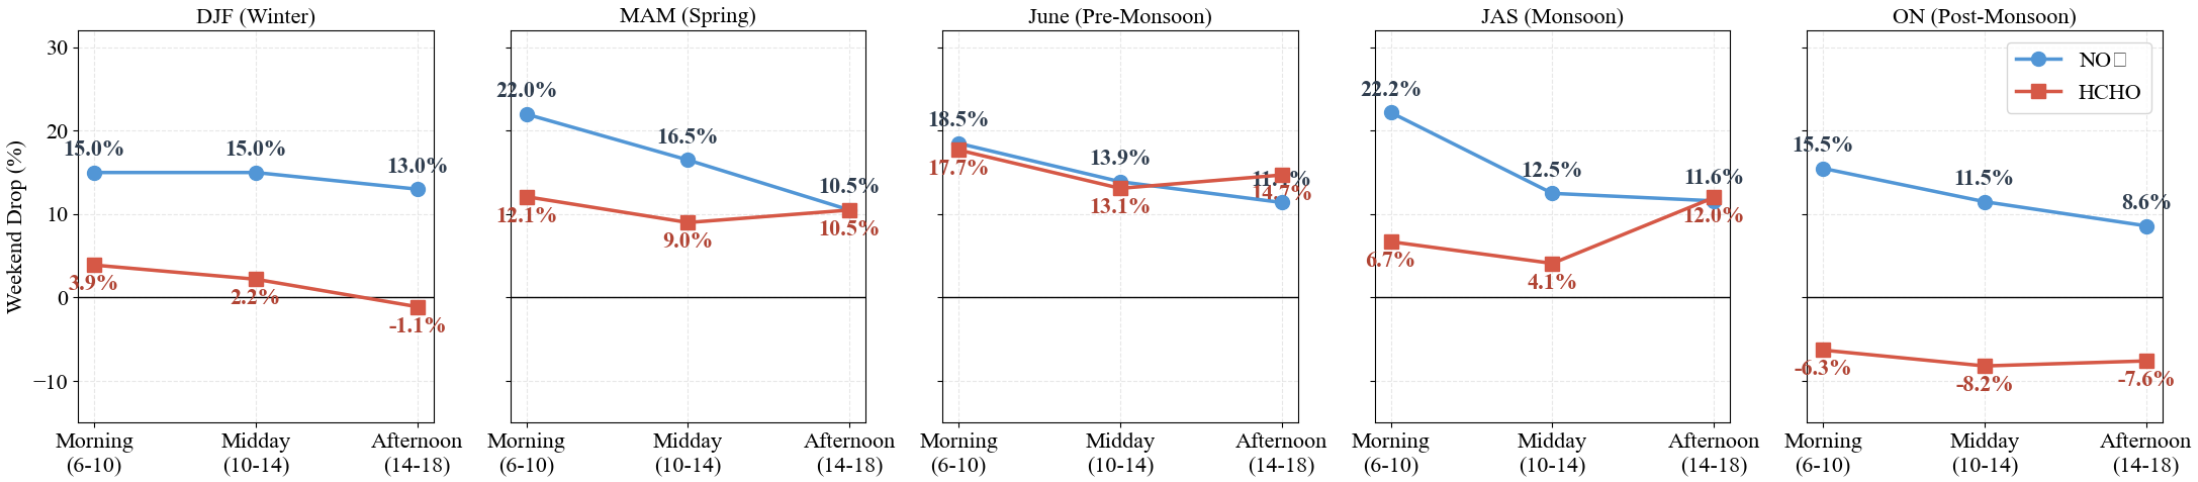
\includegraphics[width=\linewidth]{Screenshot 2026-05-16 at 8.37.34 AM.png}
    \caption{Weekend Drop by Time of Day}
    \label{fig:placeholder}
\end{figure}

\subsection{Summary}

$NO_2$ in Tucson shows a consistent traffic signal (12–17\% lower on weekends) that stays the same throughout the year. This makes perfect sense because $NO_2$ comes mainly from vehicles. The weekend drop is strongest in the morning (around 6–10 AM) when people are driving to work, and it gets weaker in the afternoon as the pollution spreads out and breaks down. No matter what season it is, $NO_2$ behaves the same way. This tells us that traffic is the main source of $NO_2$ in Tucson all year long.
$HCHO$ is different. Its weekend behavior changes drastically depending on the season, ranging from a 14.7\% drop in June all the way to an 8.2\% increase in October-November. This tells us that $HCHO$ is not just coming from traffic like $NO_2$ is. Instead, $HCHO$ possibly comes from a combination of three factors: summer chemistry, boundary layer trapping, and plants and natural sources.  

\section{Comparison with previous work}

In our findings, 12–17\% weekend drop in $NO_2$ aligns well with a study done in Pune. The paper talks about how the morning rush hour creates the strongest weekend effect \cite{BM2021B}. Due to this we can say that traffic is indeed the dominant $NO_2$ source in Tucson, just as it is in other cities.

The Pune study also found that $HCHO$ shows "no considerable difference between weekdays and weekends" \cite{BM2021B}. But we found that $HCHO$'s weekend effect varies by season, which previous studies had not specifically documented. However, we discovered that during other seasons, especially June, $HCHO$ does show a weekend effect and we also found that in post-monsoon months, $HCHO$ is actually higher on weekends. 
Our analysis of June (where $HCHO$ and $NO_2$ both drop ~17\% on weekends) reveals strong photochemical coupling between the two gases. The strong summer effect may be because of Tucson's extreme heat and clear skies during the pre-monsoon period, which creates ideal conditions for the chemical reactions that produce $HCHO$.

Like Pune, we found seasonal effects on absolute pollution levels. Winter shows lower weekday/weekend differences for $HCHO$ (only 1.3\%), probably because winter has less sunlight for $HCHO$ formation. Monsoon season shows weaker $HCHO$ weekend effects (7.4\%), similar to Pune's finding of lowest concentrations during monsoon due to less sunlight and wet climate. 

\section{Conclusions and Future works}

We analyzed data from Pandora for Tucson and found that $NO_2$ is dependent on human activity and $HCHO$ depends more on natural phenomena. Our analysis presents different perspectives and highlights different patterns across seasons, weekdays and time-of-day. We also do a comparison of the variations between pollutants. Our results match the analyses from other research.

There are a number of additional directions that we can progress in. Potential further directions include frequency domain analysis of the data. We also need to analyze multi-year data, and potentially compare the readings with data from other sources as done in \cite{HM2025}. We can compare our data with cities similar to Tucson. Finally, our hypothesis for the variations in pollutant levels has to be validated with domain experts.

    \printbibliography

\end{document}
